\subsection{Musikalische Lehrerausbildung}

\hypertarget{RefHeadingToc100333727}{}Die Entscheidung, eine Ausbildung
zum Volksschullehrer anzutreten, wurde für August Högn sicher auch
dadurch erleichtert, dass sich in der Deggendorfer Arachauergasse Nr.
94 (heutige Bräugasse Nr. 14) wenige Minuten Fußmarsch entfernt von
Augusts Elternhaus eine Präparandenschule (Abb. 6) befand. Wie zu
Volksschul-Zeiten konnte er wieder bei seinen Eltern wohnen und war
nicht mehr auf das Mettener Internat angewiesen. \footnote{Goller,
Seite 24}

Die damalige Lehrerausbildung dauerte fünf Jahre. An eine dreijährige
Vorbereitungsphase an einer Präparandenschule schloss sich die
eigentliche zweijährige Ausbildung in der Lehrerbildungsanstalt
Straubing an. Neben der Bezeichnung „Präparandenschule“, die so viel
bedeutet wie „Schule der Vorzubereitenden“, ist aus heutiger Sicht vor
allem ungewöhnlich, dass es damals gleich zwei verschiedene Schularten
gab, die vom angehenden Lehrer durchlaufen werden mussten, nämlich die
dreijährige Vorbereitungsphase an einer Präparandenschule und die
zweijährige Ausbildung in der Lehrerbildungsanstalt. Diese Tatsache
lässt sich aus der historischen Entwicklung der Lehrerausbildung
erklären. Es war Jahrhunderte lang Praxis, dass Handwerker zusätzlich
zu ihrer beruflichen Tätigkeit auch die Unterweisung der Schulkinder in
den Grundfertigkeiten wie Lesen, Schreiben und Rechen übernahmen. Die
Verordnung vom 4. September 1823 schrieb erstmals verpflichtend eine
zweijährige Ausbildung für angehende Lehrer vor und hob so
gewissermaßen den Berufsstand des Volkschullehrers im Königreich Bayern
aus der Traufe. Zuvor sollten die Anwärter drei Jahre lang bei einem
\zitat{„tüchtigen Schullehrer“ } \footnote{Lippert, Seite
153} oder einen \zitat{„vorzüglichen Geistlichen“ }\footnote{
Lippert, Seite 153} eine Art Lehre oder Praktikum ablegen, ehe man sie
ins Lehrerseminar aufnahm. Da sich diese Art der Vorbildung als nicht
effektiv herausgestellt hatte, wurde mit dem Normativ vom 29. September
1866 die dreijährige Vorbereitungszeit durch Einführung der
Präparandenschulen straffer organisiert. \footnote{Lippert, Seite 154}

Ebenso ungewöhnlich aus heutiger Sicht und kaum mit der Ausbildung der
Grund- und Hauptschullehrer vergleichbar ist die starke Gewichtung des
Musikunterrichts in der gesamten damaligen Volksschullehrerausbildung,
besonders aber in den Anfangsjahren der Präparandenschule. Das Fach
Musik – es ließ sich in die Teilbereiche \zitat{Gesang,
Violine, Klavier, Orgel }und\zitat{ Harmonielehre
}unterteilen – hatte innerhalb des Fächerkanons einen so hohen
Stellenwert, dass es neben Religionslehre, Deutsch und Rechnen
ebenfalls als Hauptfach bezeichnet wurde. \footnote{Lippert, Seite 165}
Mit 6 Wochenstunden machte der Musikunterricht mehr als ein Fünftel an
der Gesamtstundenzahl aus und zeigt deutlich die Ausrichtung der
Ausbildung, die angehenden Lehrer auf den Chorregenten- und
Organistendienst vorzubereiten. \footnote{Goller, Seite 11} Wie alle
Fächer, so wurde auch der Instrumentalunterricht von Volksschullehrern
erteilt, die an die Präparandenschule berufen worden waren.\footnote{
Goller, Seite 33} Da die Schüler vor Eintritt in die Präparandenschule
keine Vorkenntnisse im Spiel der Musikinstrumente mitbringen brauchten,
kam es oft vor, dass im Instrumentalunterricht bei einer Gruppenstärke
von durchschnittlich 10 Schülern unter den einzelnen Schülern sehr
große Leistungsunterschiede herrschten. So musste sich beispielsweise
ein fortgeschrittener Schüler, wie es August Högn im Klavierspiel war,
zusammen mit Anfängern eine Stunde teilen. Beim Klavierunterricht stand
die Hinführung auf das Orgelspiel im Vordergrund und somit die Pflege
des \zitat{„gebundenen Spiels.“}  \footnote{Goller, Seite 38}
Die Schüler sollten in der dreijährigen Ausbildung die Fähigkeit
entwickeln, leichte Sonaten und Sonatien von Bertini, Czerny, Clementi,
Dussek, und Kuhlau zu spielen. Der Orgelunterricht begann ab dem II.
Kurs, also dem 2. Schuljahr, nach Barners Schule „Anfänge des
Pedalspiels“ und bediente sich im III. Kurs der Orgelschule von
Herzog. \footnote{Goller, Seite 39} Praktische Kirchenmusikerfahrung
konnten die Schüler als Choristen unter der Woche bei der Gestaltung
von Schulmessen und an Feiertagen bei Gottesdiensten an der königlichen
Kreisirrenanstalt mit Messkompositionen der Cäcilianer Witt, Zangl,
Haberl und Ett sammeln. Sowohl die Lehrer als auch die Schüler waren
Mitglieder des Bezirk-Cäcilien-Vereins Metten und des
Pfarr-Cäcilien-Vereins Deggendorf. \footnote{Goller, Seite 47}

\begin{figure}
\centering
\img[width=5cm]{Praeparandenschule}
\caption{Gebäude der ehemaligen Präparandenschule in der heutigen
Bräugasse Nr. 14 in Deggendorf}
\end{figure}

\begin{figure}
\img{Lehrerbildungsanstalt}
\caption{Lehrerbildungsanstalt in Straubing (Ansicht gegen die
Pfarrkirche St. Jakob)}
\end{figure}

So eng die Präparandenschule und die Lehrerbildungsanstalt inhaltlich
ineinander griffen, so unterschiedlich dürfte August Högn die beiden
Schulen erlebt haben, bezüglich der Gewährung von persönlichem
Freiraum. Der seit Bestehen der Lehrerbildungsanstalt geltende
Internatszwang verliehen dem Seminar in Straubing den Charakter einer
geschlossenen Anstalt. Ein von 5 bis 21 Uhr genau festgelegter
Tagesablauf forderte von den Schülern große
Anpassungsleistungen. \footnote{Goller, Seite 61} Selbst Spaziergänge
fanden nicht ohne Aufsicht statt. Man legte großen Wert auf das
Erlernen der Fähigkeit, sich unterzuordnen, auch wenn dies nicht
explizit im Lehrplan aufgeführt war. Das hat wohl die Eingliederung der
Lehrer in die Gesellschaft an der Wende zwischen dem 19. und 20.
Jahrhundert gefördert sowie die Übernahme der Aufgaben und Pflichten,
die von dieser Gesellschaft an die Lehrer herangetragen wurden. Die
Unterordnung begünstigte aber auch wahrscheinlich die so genannte
„Untertanenmentalität“, die als ein Grund unter vielen genannt wird,
weshalb es zur Machtergreifung der Nationalsozialisten und ihrer
schrecklichen Verbrechen an der Menschlichkeit gekommen war. Wie
bereits viele Lehrer, ließ sich auch August Högn in die von den
Nationalsozialisten entworfene Gesellschaftsordnung bruchlos einordnen
und zur Übernahme von Aufgaben bewegen, die ihrerseits die Herrschaft
der Nazis unterstützten.

Während die Stundenanzahl und die Fächerverteilung im Fach Musik in etwa
mit dem Lehrplan der Präparandenschule zu vergleichen war,
unterrichteten in Straubinger Seminar nicht ehemalige Volksschullehrer
mit normaler Lehrerausbildung, sondern speziell ausgebildete Musiker.
Anton Schwarz prägte von 1892 bis 1923 das musikalische Leben an der
Lehrerbildungsanstalt maßgeblich. \footnote{Stengl, Seite 104} Er hatte
nach zwölfjährigem Volksschuldienst beim Joseph Rheinberger Komposition
und Orgel an der königlichen Musikschule in München studiert und konnte
sein erworbenes Wissen in den Fächern Harmonielehre, Orgel und Gesang
an die Schüler weitergeben. \footnote{Goller, Seite 92} Sein
umfangreiches kompositorisches Schaffen, darunter vier Messen, mehrere
Offertorien und Motetten, lieferte für manche Schüler einen Ansporn,
sich selbst im Komponieren zu versuchen. \footnote{Goller, Seite 93}

\begin{center}
\begin{minipage}{4.269cm}
\begin{flushleft}
\tablefirsthead{}
\tablehead{}
\tabletail{}
\tablelasttail{}
\begin{supertabular}{m{4.0690002cm}}

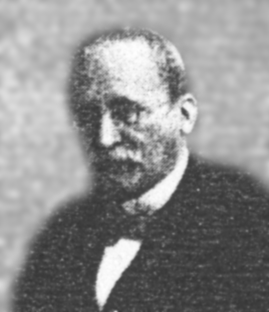
\includegraphics[width=3.886cm,height=4.531cm]{pictures/zulassungsarbeit-img010.png}

Abb. \stepcounter{Abb}{\theAbb}: Anton Schwarz\\
\end{supertabular}
\end{flushleft}
\end{minipage}
\end{center}
{\centering

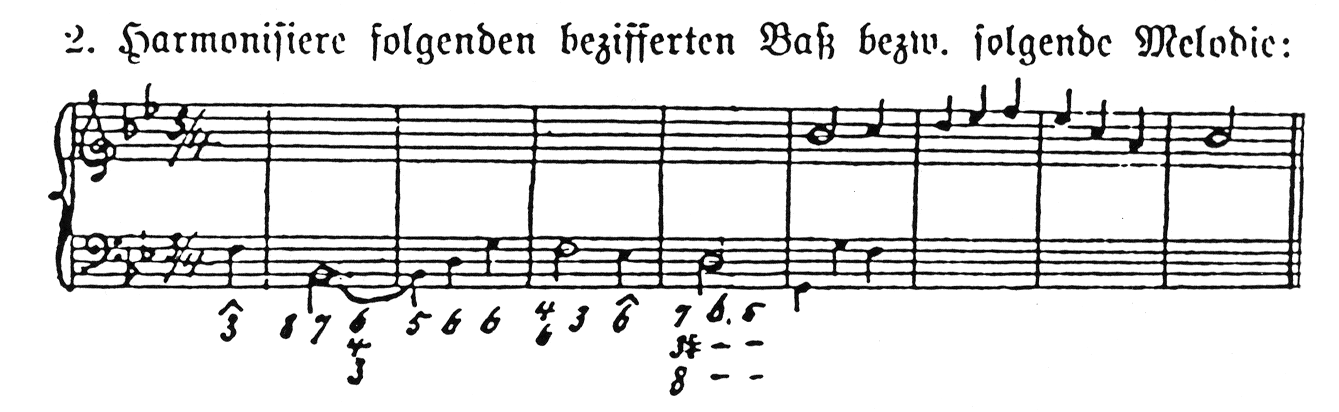
\includegraphics[width=11.088cm,height=3.258cm]{pictures/zulassungsarbeit-img011.png}
 \par}
{\centering
\label{bkm:Ref100298600}Abb. \stepcounter{Abb}{\theAbb}: Schlussprüfung
der niederbayerischen Präparandenschulen 1903
\par}

Die Schüler erhielten zwar in ihrer Ausbildung zum Lehrer keinen
Kompositionsunterricht, dafür vermittelte ihnen der
Harmonielehreunterricht die wichtigsten tonsätzerischen Regeln, mit
denen sie in Eigenregie erste kompositorische Schritte wagen konnten.
Wie die im Fach Harmonielehre gestellten Prüfungen zeigen (Abb. 9),
gehörte das Umgehen mit dem vierstimmigen Chorsatz zu dem Handwerkszeug
eines angehenden Lehrers. Man kann deshalb August Högns Werke – sie
haben mit wenigen Ausnahmen den vierstimmigen Satz als Grundgerüst –
als Früchte des Musikunterrichts der Lehrerausbildung
betrachten. \footnote{Goller, Seite 74}
